\chapter{需求分析}

本章针对AI多任务调度系统现状的三大问题（对AI相关特性的适配不佳、无法判断AI任务是否具备执行条件、无法识别AI多任务场景下的资源互斥）进行了分析，并明确了对应的功能需求。

\section{AI多任务场景问题分析}

在人工智能大模型技术快速演进的背景下，传统的任务编排与调度模式已难以适配AI任务高算力、长周期及多模态数据交互等核心特征。早期系统架构多围绕“固定流程执行”设计，核心目标是处理逻辑单一、计算资源需求可预见的批处理作业，在处理大规模异构AI任务时暴露出严重的滞后性。

在适配性维度上，现有调度系统因缺乏对AI任务特性的深度感知，面临数据治理难度高与操作链路冗余的双重挑战。AI任务涉及海量Prompt模板与异构模型参数，由于缺乏标准化参数画像约束，手工录入过程中频发全角/半角符号混用或非法字符干扰，严重削弱了模型的响应质量与语义一致性。同时，由于系统缺乏针对输入数据的自动纠偏机制（如浮点数与整数的自动转换或类型推断能力），细微的数据偏差易引发任务的崩溃，导致系统鲁棒性显著不足。此外，任务中断后的参数重校与重启高度依赖人工干预，未能构建端到端的自动化调度闭环，显著推高了系统的运维成本与操作复杂度。

在调度决策维度，现有系统因缺乏对内外部环境的自主感知能力，导致调度流程高度依赖人工干预。目前启动决策机制较为单一，多采用手动触发或固定时序模式，无法实时感知系统负载变化或匹配特定的运营策略，在资源峰值期间极易引发请求雪崩。此外，在缺乏逻辑引擎支持的情况下，系统难以对网络抖动、内存不足等环境异常进行自主判别与自愈，无法形成自动化的调度闭环。

在资源互斥识别维度，针对GPU等昂贵且稀缺的计算资源，现有系统由于缺乏细粒度的冲突分析能力，造成了严重的算力资源浪费。AI任务对核心资源（如GPU显存）具有强独占性特征，但传统调度层无法精准识别任务间的资源依赖拓扑，导致多个任务在抢占同一临界资源时频发数据错乱或运行失败。由于无法有效识别任务间的互斥状态，运维层面往往被迫采取保守的串行执行策略，这种“调度黑盒”限制了系统的并发吞吐量，使高价值算力资源在任务间隙处于闲置状态，成为制约AI研发效能提升的关键瓶颈。

综上所述，当前调度体系在适配AI任务异构特性、环境感知自动化以及高价值算力资源精细化管控方面存在显著的技术缺位。这些瓶颈不仅导致了研发流程中严重的数据治理难度与人力冗余，更因调度逻辑的滞后性制约了计算资源的利用效率。

\section{AI多任务资源调度系统总体目标}

为有效解决当前AI任务管理中适配性欠缺、决策自动化程度低及资源互斥识别不足三大挑战，本文设计并实现了一套面向AI场景的资源调度系统，旨在通过技术手段提升大模型研发效能。系统设计的总体目标涵盖以下三个核心维度：

强化任务深度适配与数据鲁棒性。通过构建标准化分组管理机制与异构数据映射机制，实现任务、资源及附件的精细化隔离。引入智能参数校验与自动纠偏逻辑，针对参数录入中的格式差异与语法偏差进行实时修正，旨在解决异构环境下数据处理能力不足的问题，显著降低系统的操作复杂度。

实现调度决策的环境感知与去人工化。系统依托业务逻辑引擎构建任务可用性分析机制，通过对系统负载与运营策略的实时感知，实现调度指令的自主下发与执行决策。操作员无需手动干预任务启动时机，配合批量化控制功能，旨在消除重复性机械劳动，提升任务流转的自动化水平。

优化临界资源管控精度与并发执行效率。通过设计针对GPU等稀缺资源的互斥智能分析算法，精准识别任务间的资源依赖拓扑，从而打破传统模式下的串行启动限制。结合腾讯基础设施的全面监控能力，实现对任务运行状况与算力占用的精准捕获，最大化计算集群的利用率与系统吞吐量。

此外，系统以分组为基本维度建立严密的鉴权体系，并配置完善的异常恢复机制。在性能维度，利用分布式架构与异步并发技术，确保系统具备毫秒级的调度响应与高吞吐处理能力；在稳定性维度，通过多维度的实时监控与多级容错策略，赋予系统在计算过载与网络抖动场景下的自愈能力。在确保数据安全、系统鲁棒与运行高效的同时，全方位提升AI多任务场景下的管理效能

\section{API接入层功能需求分析}

本系统采用前后端分离架构，重点阐述后端服务器及调度执行队列的实现方式，对前端系统不予赘述。在前后端分离模式下，前端通过HTTP请求访问后端API接口。本节将剖析系统在API接入层面临的挑战，重点针对子问题一提出的AI特性适配不佳及异构数据校验难题展开分析。此外，由于系统部署于公司内网且涉及昂贵的AI算力资源，API层必须建立严密的鉴权机制以规避误操作与潜在的数据泄露风险。本节将给出涵盖任务控制、权限鉴定及数据自动纠偏在内的具体需求分析。

\subsection{任务的创建、修改和撤销}

任务生命周期管理（涵盖创建、修改及撤销）是调度系统的核心功能组件。本系统将相关功能划分为“任务脚本管理”与“任务实例控制”两个维度。在脚本管理维度，为保障AI逻辑的安全性与系统稳定性，操作员上传或修订Python脚本后需进入审核流程，经部门管理员审批通过后方可上线执行。在实例控制维度，操作员可基于Web端直接完成任务创建、参数配置及撤销操作。由于此类操作主要针对具体的任务运行参数且时效性要求较高，其影响范围相对受限，故不设置冗余的审核环节，旨在平衡系统安全性与运维灵活性。本系统中，任务相关的用例图如图3.1所示。

\begin{figure}[htbp]
    \centering
    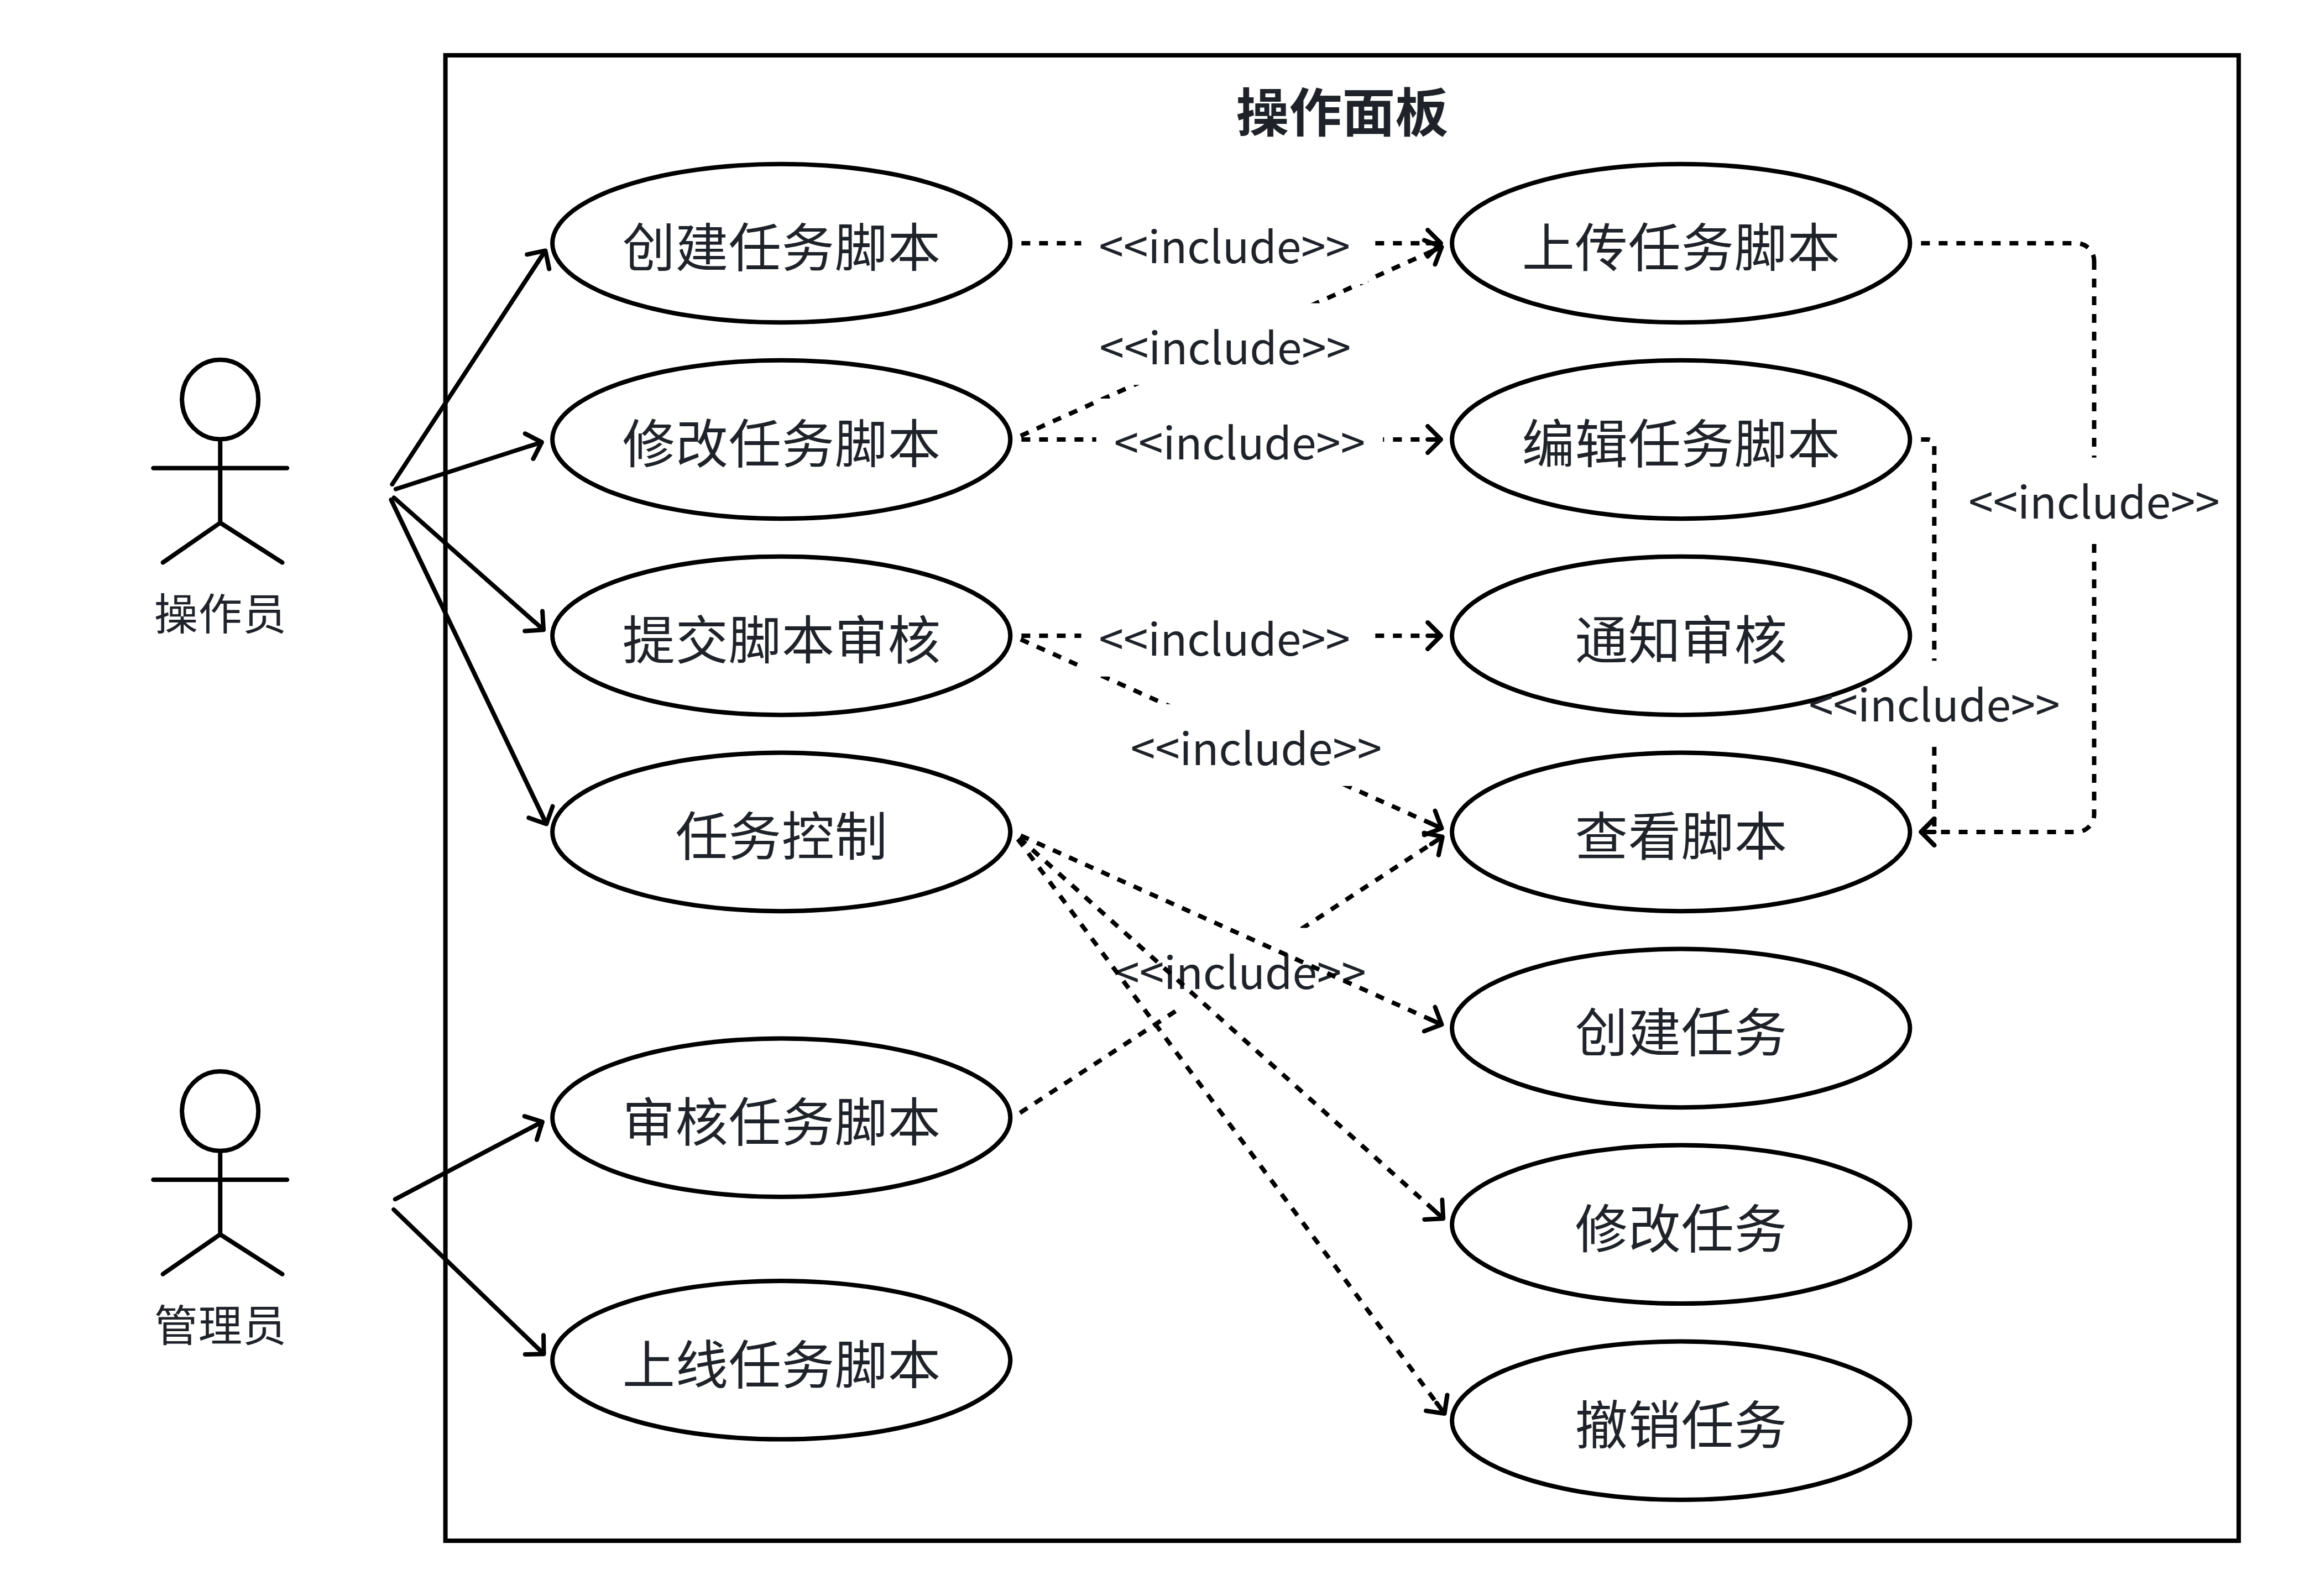
\includegraphics[width=\linewidth]{figures/3/任务操作用例图.png}
    \caption{任务操作用例图}
    \label{fig:enter-label}
\end{figure}

\subsection{权限鉴定}

本系统部署于公司内网环境，为有效防范误操作并规避潜在的数据泄露风险，必须建立严密的身份鉴权与访问控制机制。此外，针对开源生态中的版权归属困境及行业合规管理要求，系统需通过细粒度的权限策略确保安全合规。本系统设计了基于“任务组”的权限模型，将用户划分为系统管理员与操作员两类角色：

\begin{enumerate}
    \item 系统管理员：拥有全局最高权限，负责任务分组的创建、资源配置及对操作员的授权管理。
    \item 操作员：在获得对应任务组授权后，可独立执行任务实例的创建、修改及撤销操作。为强化逻辑安全性，操作员发起的脚本上传或代码修订须经管理员审批通过后方可生效。
\end{enumerate}

这种分层授权的设计模式，既通过管理员的审批把控保障了系统核心逻辑的安全，又赋予了操作员在授权范围内自主处理任务的灵活性，有效平衡了安全管控与运维效率。本系统的权限系统用例图如图3.2所示。

\begin{figure}[htbp]
    \centering
    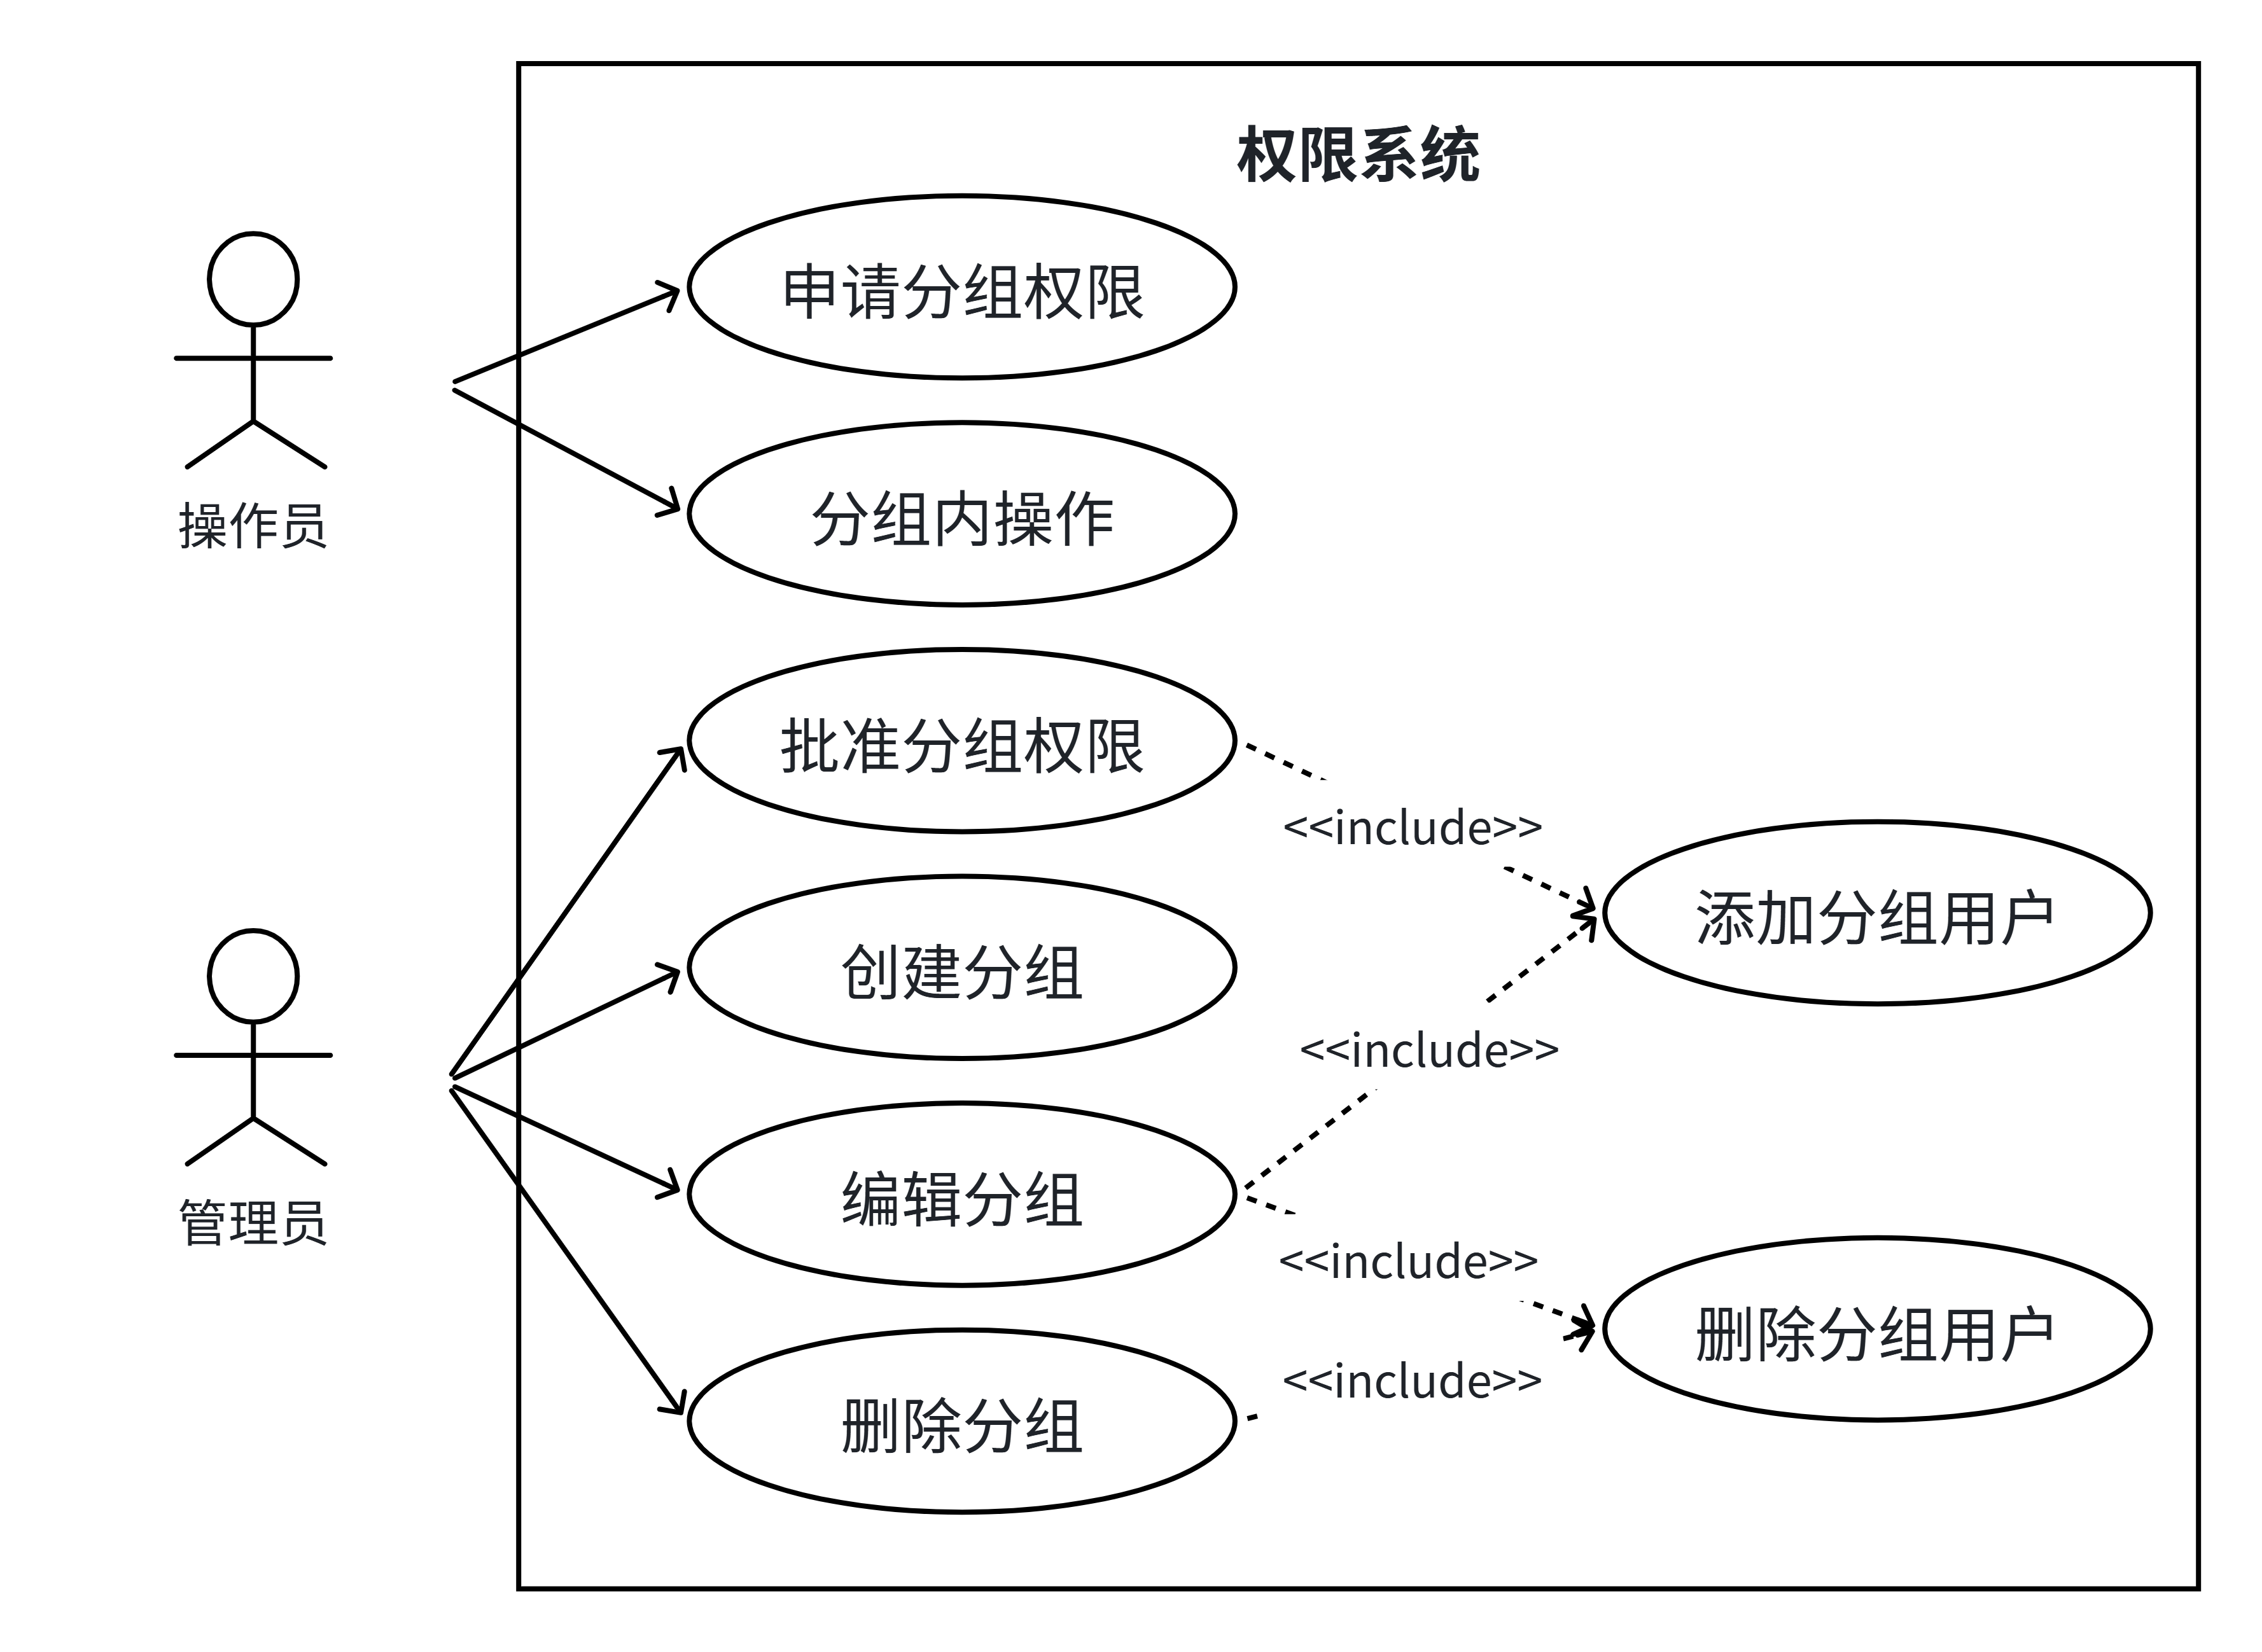
\includegraphics[width=\linewidth]{figures/3/权限系统用例图.png}
    \caption{权限系统用例图}
    \label{fig:enter-label}
\end{figure}

\subsection{数据校验与自动纠正}

为有效解决子问题一中提到的系统对AI特性适配不足及数据处理能力匮乏的问题，API接入层须具备深度的数据感知与鲁棒性纠偏能力。针对AI多任务场景下参数异构、格式复杂的特点，本系统构建了双层校验与修正机制，旨在从源头保障数据的准确性与一致性。

异构数据类型过滤与标准化校验。鉴于Python作为动态类型语言在编译期缺乏强制约束，系统引入了基于Pydantic库的数据验证层。通过建立大模型任务参数画像，对API请求实施实时结构化扫描，强制约束Prompt模板及模型超参数等字段符合预定义的Schema规范，从底层规避因类型不匹配导致的任务崩溃风险。

特定参数自动化纠偏机制。针对操作员录入过程中高发的非致命性逻辑偏差，系统设有智能纠正模块以提升交互容错性。具体包括：自动将全角标点转化为标准半角字符以适配列表处理；识别并剔除复制粘贴产生的冗余括号符号；以及在不损失数值精度的前提下实现浮点数向整数的自动推断与转化。

数据鲁棒性与运维效能优化。该机制通过在接入端预先拦截并修复格式偏差，显著降低了系统的操作门槛与无效请求的重试频率。这不仅保障了下行至调度层与执行层数据的纯净度，也为后续实现复杂的自动化调度闭环奠定了可靠的数据基础。

本需求相关用例如表3.1所示。

\begin{table}[htbp]
\centering
\caption{数据校验与自动纠正功能用例表}
\begin{tabularx}{\textwidth}{lllXl}
\toprule
\textbf{用例ID}&\textbf{用例名称}&\textbf{处理类型}&\textbf{核心操作}&\textbf{处理结果}\\
\midrule
UC-DV-001&AI参数画像匹配&校验&匹配Prompt/超参数Schema&合法通过\\
UC-DV-002&异构类型校验&校验&基于Pydantic实施类型检查&合法通过\\
UC-DV-003&全角标点纠偏&纠正&全角符号向半角标点转化&修正通过\\
UC-DV-004&冗余符号清理&纠正&剔除冗余括号空格等&修正通过\\
UC-DV-005&数值类型推断&纠正&浮点数向整数无损转化&修正通过\\
UC-DV-006&字符串格式化&纠正&去除首尾空格及不可见字符&修正通过\\
UC-DV-007&日期格式统合&纠正&统一日期字符串为“YYYY-MM-DD”&修正通过\\
UC-DV-008&校验结果反馈&反馈&汇总校验报告并下发提示&返回报告\\
\bottomrule
\end{tabularx}
\label{tab:data_validation_cases}
\end{table}

\section{任务调度层功能需求分析}

任务调度层作为本系统的核心逻辑中枢，承担着从任务接入到分发执行之间的关键决策与协调职能。任务调度和资源分配是与服务稳定性、用户满意度以及资源利用率直接相关的两个主要问题\cite{pan2025}。本章将深入剖析该层的功能需求，旨在通过技术手段解决人工智能多任务场景下的自动化决策与算力资源治理难题，具体需求如下：

环境感知的自动化决策：改变传统模式下过度依赖人工判断任务启动时机的现状。系统需具备任务可用性检测功能，通过逻辑引擎实时感知系统负载与运营策略，自主判定任务执行条件，消除调度过程中的人工干预环节。

算力资源的精细化管控：针对GPU等昂贵且稀缺的AI临界资源，系统需建立完备的资源可用性检测机制。通过识别任务间的资源依赖拓扑，精准处理资源互斥冲突，打破传统“保守串行”的限制，在保障数据安全的前提下实现高效的并发调度。

保障分布式环境下的稳健运行：面对异构集群带来的性能差异，系统需支持智能负载均衡，通过权重轮询等算法优化算力分配。同时，构建可靠的数据同步机制与容错恢复体系，确保在网络抖动或算力过载等异常场景下，任务流程依然具备强劲的鲁棒性与自愈能力。

通过上述功能维度的深度分析，本层将建立起一套覆盖智能感知识别、资源动态博弈与高可用性保障的调度体系，为AI研发效能的提升提供坚实支撑。

\subsection{任务可用性检测}

针对子问题二中“调度决策过度依赖人工判断”导致的效能瓶颈，系统需建立具备环境感知能力的自动化决策体系。本系统定义的AI任务在底层实现上表现为支持动态编辑与更新的Python函数，通过调用大模型接口协同输入数据完成特定业务功能。

在传统调度模式下，任务启动时机完全取决于操作员的人工经验，难以精准应对高动态的系统负载环境，系统亟需构建一套基于环境感知策略驱动的逻辑引擎，以解决人工判断的局限性。该引擎需支持管理员通过预设的配置规则（如系统负载阈值、特定场景约束等），将复杂的运营策略转化为可自动执行的决策逻辑。通过这种方式，系统能依据实时负载动态判定任务的执行可行性，实现调度权力由“人工干预”向“引擎自决”的自动化转型，从而在保障业务连续性的同时，显著提升多任务环境下的全局调度效能。本需求的用例表如表3.2所示。

\begin{table}[htbp]
    \centering
    \caption{任务可用性检测功能用例表}
    \begin{tabular}{llll}
        \toprule
        \textbf{用例ID} & \textbf{用例名称} & \textbf{核心操作} & \textbf{处理结果} \\
        \midrule
        UC-TA-001 & 系统负载检测 & 实时采集系统负载值 & 输出负载状态 \\
        UC-TA-002 & 负载阈值配置 & 管理员设置负载阈值 & 保存配置生效 \\
        UC-TA-003 & 任务启动判断 & 对比负载与阈值 & 允许/禁止启动 \\
        UC-TA-004 & 高负载任务限制 & 过载时拦截高耗任务 & 拦截并提示 \\
        UC-TA-005 & 配置修改记录 & 保存管理员配置操作 & 生成操作日志 \\
        UC-TA-006 & 异常场景触发 & 节假日等场景激活规则 & 自动启用限制 \\
        UC-TA-007 & 任务拦截反馈 & 告知用户拦截原因 & 提示负载过高 \\
        UC-TA-008 & 负载回落恢复 & 负载低于阈值时 & 恢复任务启动 \\
        \bottomrule
    \end{tabular}
    \label{tab:task_availability_cases}
\end{table}

\subsection{资源可用性检测}

针对子问题三中“因缺乏资源互斥智能分析能力致使任务盲目串行、算力利用率低下”的痛点，系统需构建精细化的资源感知与管控机制。AI任务在执行过程中对高性能算力资源（如GPU显存、专用硬件等）具有强独占性特征。若两个任务试图同时调用同一临界资源，将引发严重的资源抢占冲突，导致数据错乱或运行失败。

为此，本系统需设计一套基于资源拓扑识别的互斥智能分析机制，以取代传统低效的保守调度策略。首先，系统需建立完备的资源注册体系，强制要求任务在提交时声明其所需的临界资源清单。其次，调度层需具备动态分析能力，通过计算在途任务间的资源依赖拓扑，精准识别各任务间的互斥状态。若判定任务具备执行条件（即目标资源空闲且无互斥冲突），系统应立即触发并发调度；若检测到资源冲突，则需将其加入高可靠等待队列，直至临界资源释放后由调度器自动唤醒。通过这种精细化的资源管控，旨在打破传统模式下的串行执行瓶颈，将调度逻辑由“保守串行”向“安全并发”转变，从而显著压低算力资源的闲置率，提升系统整体吞吐性能。本需求的用例表如表3.3所示。

\begin{table}[htbp]
    \centering
    \caption{资源可用性检测功能用例表}
    \begin{tabular}{llll}
        \toprule
        \textbf{用例ID} & \textbf{用例名称} & \textbf{核心操作} & \textbf{处理结果} \\
        \midrule
        UC-RA-001 & 资源提前注册 & 任务声明所需资源并登记 & 资源信息入库 \\
        UC-RA-002 & 任务资源声明 & 任务提交时标注资源需求 & 记录任务-资源关联 \\
        UC-RA-003 & 任务互斥判定 & 比对任务所需临界资源 & 识别互斥任务 \\
        UC-RA-004 & 执行权限判断 & 检查目标资源占用状态 & 允许/拒绝执行 \\
        UC-RA-005 & 任务等待入队 & 无资源时标记任务状态 & 加入资源等待队列 \\
        UC-RA-006 & 资源释放监测 & 实时跟踪资源占用变化 & 捕获资源空闲状态 \\
        UC-RA-007 & 等待任务唤醒 & 资源空闲时触发队列调度 & 唤醒等待任务执行 \\
        UC-RA-008 & 互斥冲突提示 & 告知用户任务互斥原因 & 提示资源被占用 \\
        \bottomrule
    \end{tabular}
    \label{tab:resource_availability_cases}
\end{table}

\subsection{负载均衡及性能优化}

在本系统分布式架构中，任务执行节点(Worker)表现出显著的硬件与软件异构性。受限于物理基础（如CPU核心、内存容量及I/O吞吐）、运行环境（OS版本、依赖库差异）以及部署策略的不同，各节点间的算力输出与资源偏好天然存在差异。例如，搭载高性能GPU的节点专精于大模型推理，而普通节点则侧重于通用逻辑处理，资源配置重心截然不同。若沿用传统的均等化调度模式，不仅无法有效适配节点间的算力差异，还容易导致高价值资源在峰值期间被无效抢占，进一步加剧了子问题三中提到的算力浪费与任务阻塞难题。

为突破上述瓶颈，系统需构建一套基于实时状态感知与任务需求建模的负载均衡机制。该机制要求调度层精准采集各Worker的实时负载指标（涵盖CPU/内存利用率、队列长度及剩余算力评估），并动态分析各类AI任务的资源亲和性特征。通过引入智能权重分配算法，系统应实现任务与节点的最佳匹配：将计算密集型训练或推理任务优先指派至算力充裕的GPU节点，而将参数处理等轻量级任务分发至响应及时的通用节点。这种精细化的调度方案不仅能有效规避单点过载引发的任务堆积，更能充分释放异构集群的算力潜力，确保在应对多任务高并发场景时，系统始终保持高吞吐与低延迟的稳健运行状态。

\subsection{数据同步}

在分布式AI调度体系中，任务流转涉及复杂的Prompt模板、模型超参数及大规模异构中间数据。子问题一明确指出，现有系统对AI特性的适配性不足，主要体现在异构参数处理与数据类型分析能力的缺失上。若各子模块（如任务创建、执行、存储模块）间的数据同步机制存在缺陷，API接入层预先完成的参数纠偏与类型推断结果将无法准确、完整地透传至任务执行节点。这种数据流转过程中的失真与偏差，不仅会导致任务执行逻辑偏离预设轨道，产生与实际需求相悖的无效结果，更会因频繁的数据回溯与重复执行而造成高昂算力资源的严重浪费。

为攻克适配性难题，系统亟需构建一套高可靠、强一致的数据同步机制，作为保障AI任务顺畅推进的核心支撑。该机制需深度对接大模型任务参数画像，确保异构数据映射结果与自动纠偏策略在任务生命周期的各阶段保持实时一致。当任务在不同子模块间流转时，系统必须保障Prompt配置、中间计算结果及执行状态标识的高度同步，消除因子模块数据差异导致的决策瓶颈。通过建立基于高性能中间件的消息同步底座，系统旨在实现数据的透明流转与闭环管理，为任务的稳定运行及后续的算力精准调度提供坚实的数据基础。

\subsection{容错与恢复}

针对系统适配性欠佳及异构数据处理能力不足的问题，系统需构建完善的容错与自动化恢复机制，以保障AI任务在复杂生产环境下的性能表现与持续稳定性。AI任务普遍具有高算力消耗与执行周期长的特征，任何非预期的流程中断都会造成昂贵计算资源的无效浪费。因此，系统应具备对非致命性异常的动态识别与自助修复能力，通过重试逻辑或参数自动纠偏手段完成初步恢复。在确保任务连续性的同时，系统需实现异常处理的静默化，从而最大限度降低操作员的运维频率与心智负担。结合生产环境的实际需求，系统需重点针对以下两类异常场景建立自愈策略：

\begin{enumerate}
    \item 网络通信韧性保障：尽管系统部署于公司内网，但由于内网拥堵引发的超时风险依然存在。系统需将超时视为典型的可恢复异常，并依据预设规律（如指数退避机制）进行自动重试。这不仅能保障调度响应的及时性，还能有效增强系统在复杂网络环境下的运行韧性。
    \item 数据类型自愈与纠偏：受分布式架构中子模块版本更新不及时等因素影响，系统常遭遇异构数据传输导致的参数错误，如浮点数（float）与整数（int）类型冲突。基于子问题一的适配性要求，系统需内置智能纠偏规则，对简单的类型不匹配、字符输入偏差（如全角/半角标点混用）或逻辑拼写失误进行实时修复与无损转化，确保下行指令的准确性与鲁棒性。
\end{enumerate}

通过建立多级容错恢复体系，系统旨在实现从“人工排查异常”向“系统自动感知与治理”的深度转型，从根本上解决调度流程中的性能瓶颈与稳定性隐患。

\section{任务执行层功能需求分析}

本系统采用分布式微服务架构，任务执行层作为算力调度的最终落地单元，需直接面对AI大模型任务高算力、长周期及数据异构等核心特征。针对现有调度体系在AI特性适配性上的局限，以及对异构数据处理与类型分析能力的不足，本层通过构建标准化的参数传递协议、灵活的任务编辑机制以及深度的异常捕获流程，确保API接入层完成的参数纠偏与数据画像结果能够精准转化为算力输出。在这种独特的部署模式下，如何保障复杂AI参数在跨节点传输时的准确性，以及在执行过程中对资源占用的即时响应，衍生出了以下关键功能需求。接下来，本章将深入剖析这些功能需求的具体内容及其设计的必要性。

\subsection{参数传递}

基于系统灵活性与可扩展性的工程考量，本系统采用分布式微服务架构，将“任务调度层”与“任务执行层”解耦部署于不同的计算节点。在这种物理隔离的架构下，AI任务指令与超参数无法通过传统的本地函数调用进行交互，必须依赖复杂的网络环境完成跨节点传输。针对现有调度体系在AI异构数据处理及环境适配能力上的缺失，执行层在接收参数后需建立一套深度适配机制，无法直接投入计算。由于深度学习算法具有极强的数据依赖性，系统必须在任务启动前执行参数预处理逻辑。例如，需自动化完成大规模远程附件的并发拉取，并动态执行参数画像中的路径重定向，将远程URL映射为本地物理路径，以确保任务脚本在异构执行环境下的逻辑一致性。为确保AI异构参数在分布式环境下的高效流转，本系统在参数传递环节需满足以下核心需求：

\begin{enumerate}
	\item 透明传输：对于操作员以及本系统的各个子模块而言，在参数的发送与接收过程中，应实现无感操作，就如同进行本地系统调用一般。为此，本层需具备支持任意类型和大小参数的能力。
	\item 可靠传输：本系统需确保参数传递的准确性。因为传递错误的参数极有可能致使任务出现异常，进而导致结果无效。此外，系统还应保障任务与参数能够可靠传达，即能够及时察觉任务丢失问题，并采取重试措施。
	\item 远程附件拉取：部分任务依赖远程附件，对此，本系统需预先准备好这些附件，并将对应的参数修改为本地路径，以便任务能够无感知地读取附件。
\end{enumerate}

本系统参数传递功能用例表如表3.4所示。

\begin{table}[htbp]
    \centering
    \caption{参数传递功能用例表}
    \begin{tabular}{llll}
        \toprule
        \textbf{用例ID} & \textbf{用例名称} & \textbf{核心操作} & \textbf{处理结果} \\
        \midrule
        UC-PT-001 & 参数封装处理 & 打包任意类型参数 & 生成传输数据包 \\
        UC-PT-002 & 透明传输处理 & 屏蔽网络传输细节 & 实现无感调用 \\
        UC-PT-003 & 传输校验机制 & 验证参数完整性 & 确保数据准确 \\
        UC-PT-004 & 任务丢失检测 & 监控传输状态 & 发现丢失触发重试 \\
        UC-PT-005 & 远程附件拉取 & 下载远程附件至本地 & 生成本地文件路径 \\
        UC-PT-006 & 参数路径替换 & 将远程路径改为本地路径 & 适配本地执行环境 \\
        UC-PT-007 & 断点续传支持 & 大参数分片传输 & 支持中断后继续 \\
        UC-PT-008 & 传输结果反馈 & 返回参数处理状态 & 告知成功/失败原因 \\
        \bottomrule
    \end{tabular}
    \label{tab:parameter_transfer_cases}
\end{table}

\subsection{任务编辑}

在AI大模型任务的实际执行过程中，面对参数空间呈指数级增长的调优需求，以及业务指标随环境波动而产生的高度不确定性，受限于模型超参数的复杂性以及业务需求的动态演进，操作员常需对已提交或正在运行的任务进行参数微调或类型修正。然而，传统的调度模式往往缺乏对执行中任务的即时干预能力，使得系统极易陷入“预设指令”与“实际需求”脱节的僵化状态。

若无法实现任务的动态编辑，将导致由于操作疏忽引发的错误逻辑持续空耗昂贵的计算资源，甚至造成核心算力集群的长效阻塞。因此，任务执行层必须构建一套高可靠的撤销与重启机制。这不仅是为了赋予操作员灵活的容错纠偏能力以回应数据适配挑战，更是为了确保在变更发生时，能够通过对底层进程的精细化治理，即时终止异常进程并释放被独占的GPU等临界资源，从而最大化算力周转效率，避免无效负载对硬件寿命与研发周期的双重损耗。同时，重启后的新任务必须重新联动自动化决策引擎，结合当前集群的负载实况与策略权重，重新判别其是否满足最新的执行条件。
具体的撤销与重启机制需满足以下几点要求：

\begin{enumerate}
	\item 及时终止对应进程：在AI系统中，算力资源极为宝贵。因此，及时终止旧进程以节约算力，显得尤为重要。
	\item 及时释放对应资源：本系统存在诸多仅能互斥使用的资源。及时释放这类资源，有助于提高本系统的并发处理能力，缩短其他任务的执行周期，进而提升系统吞吐量。
	\item 判断新任务是否满足运行要求：旧任务撤销后，新任务启动需满足本系统的两个条件：其一，依据运营策略计算得出任务可执行；其二，任务所依赖的资源未被占用。本系统需在发送新任务前，重新进行上述计算。
\end{enumerate}

本系统任务编辑功能用例表如表3.5所示。

\begin{table}[htbp]
    \centering
    \caption{任务编辑功能用例表}
    \begin{tabular}{llll}
        \toprule
        \textbf{用例ID} & \textbf{用例名称} & \textbf{核心操作} & \textbf{处理结果} \\
        \midrule
        UC-TE-001 & 任务撤销触发 & 接收操作员撤销指令 & 启动终止流程 \\
        UC-TE-002 & 任务参数修改 & 编辑任务参数及类型 & 保存修改内容 \\
        UC-TE-003 & 任务重启执行 & 符合条件时启动新任务 & 任务进入运行态 \\
        UC-TE-004 & 操作结果反馈 & 返回撤销/重启状态 & 告知成功/失败原因 \\
        \bottomrule
    \end{tabular}
    \label{tab:task_editing_cases}
\end{table}

\subsection{异常捕获}

本系统在任务执行过程中，可能会遭遇多种异常情况，诸如k8s的CPU Limit（即CPU受限）问题、内存受限问题等。以系统迭代过程中的一个真实案例为例，操作员上传了一段存在问题的Python代码。此代码包含发送数据包的业务逻辑，但在完成数据包发送后，却未及时关闭相应的文件描述符（file descriptor）。结果在数小时内，系统内存占用量持续攀升，最终引发异常，导致操作员前期投入的工作成果失效。该案例将在后续“系统测试与分析”章节中详细阐述，在此提及旨在表明，本系统有必要设计一套异常捕获机制。借助这一机制，能够及时监控并分析系统出现的异常状况，及时上报异常信息并尝试恢复系统正常运行，这将极大地节省操作员的工作量，有效提高工作效率。本系统的异常捕获与恢复机制，需要满足如下几点要求：
\begin{enumerate}
	\item 全面且细致地监测系统各项指标，针对诸如CPU、内存、文件描述符等易对系统稳定性产生影响的关键指标，构建基于历史数据的预测机制。一旦发现问题，即刻通知相关人员。如有必要，及时暂停相关任务，并暂存相关数据，以此避免数据丢失及工作量的浪费。
	\item 异常信息采集：依托Python的异常处理流程，本系统能够构建一套完备的异常信息采集机制。当任务出现异常时，系统应及时采集异常信息，并通知相关人员。详尽的异常信息有助于相关人员分析错误原因，进而修复错误，及时止损并促使系统恢复正常运行。
\end{enumerate}

这不仅将极大地减轻操作员的人工值守负担，将从繁琐的故障排查中解放出来，更能有效保障昂贵计算资源的周转效率，从而在整体工程维度上实现开发与运维效率的跨越式提升。

本系统异常捕获功能用例表如表3.6所示。

\begin{table}[htbp]
    \centering
    \caption{异常捕获功能用例表}
    \begin{tabular}{llll}
        \toprule
        \textbf{用例ID} & \textbf{用例名称} & \textbf{核心操作} & \textbf{处理结果} \\
        \midrule
        UC-EC-001 & 系统指标监测 & 实时采集CPU/内存/文件描述符 & 输出指标数据 \\
        UC-EC-002 & 异常预测预警 & 识别指标异常 & 触发预警通知 \\
        UC-EC-003 & 异常任务暂停 & 终止目标任务 & 避免资源浪费 \\
        UC-EC-004 & 任务数据暂存 & 暂停任务前保存中间数据 & 防止数据丢失 \\
        UC-EC-005 & 异常捕获 & 异常流程采集信息 & 获取异常日志 \\
        UC-EC-006 & 异常信息上报 & 推送详情至相关人员 & 通知处理故障 \\
        UC-EC-007 & 异常原因分析 & 整理数据辅助排查 & 提供分析依据 \\
        UC-EC-008 & 系统恢复尝试 & 重启服务释放资源 & 恢复系统运行 \\
        \bottomrule
    \end{tabular}
    \label{tab:exception_capture_cases}
\end{table}

\section{非功能需求}

非功能需求作为系统构建的重要基石，不仅决定了资源调度系统在工业生产环境中的可用边界，更是支撑本文核心研究目标——解决AI多任务场景下适配、决策与资源利用三大瓶颈的关键所在。

具体而言，高性能特性是实现算力资源高效并发调度与动态周转的技术先决条件，直接决定了系统在应对大规模 AI 任务时资源利用率的上限；工业级稳健性则是驱动调度决策机制由传统人工干预向全自动化、自愈式演进的核心保障，确保系统在面临硬件失效或网络波动等极端工况时，仍能维持业务逻辑的持续性与系统状态的一致性；而广泛的兼容性则确保了参数传递机制在分布式异构底座上的逻辑一致性，为系统的规模化工业推广及研发效能的提升提供了底层支撑。

\subsection{性能需求}

系统应具备高并发环境下的实时请求处理能力，核心在于解决子问题三中算力资源利用率低下的痛点。通过将资源互斥智能分析与调度决策的响应延迟控制在极低阈值内，实现对AI算力资源的高效并发周转，旨在消除传统串行模式引发的调度瓶颈。同时，系统在执行批量控制指令与大规模附件流转时需保持高度流畅，以适配AI高频研发场景，确保无明显感知卡顿。根据量化性能指标要求，在10并发的常规工况下，任务提交、删除及编辑的平均响应时间应低于50ms；在100并发的中等压力下，响应时间应控制在100ms以内；即便在1000并发的极端高负载场景下，平均响应时间也需限制在500ms以内且确保系统稳定运行无崩溃。这一性能表现将从技术底层保障子问题二中自动化决策引擎的执行效率，支撑大规模AI任务的快速流转。相关参数需求指标如表3.7所示。

\begin{table}[htbp]
\centering
\caption{性能需求指标表}
\begin{tabular}{lll}
\toprule
测试内容 & 预期结果 \\
\midrule
10 并发下提交任务平均响应时间 & 响应时间 < 50 ms \\
10 并发下删除任务平均响应时间 & 响应时间 < 50 ms \\
10 并发下编辑任务平均响应时间 & 响应时间 < 50 ms \\
100 并发下提交任务平均响应时间 & 响应时间 < 100 ms \\
100 并发下删除任务平均响应时间 & 响应时间 < 100 ms \\
100 并发下编辑任务平均响应时间 & 响应时间 < 100 ms \\
1000 并发下提交任务平均响应时间 & 响应时间 < 500 ms \\
1000 并发下删除任务平均响应时间 & 响应时间 < 500 ms \\
1000 并发下编辑任务平均响应时间 & 响应时间 < 500 ms \\
\bottomrule
\end{tabular}
\label{tab:perf_concurrent}
\end{table}

\subsection{稳定性需求}

系统需保障工业级的长期运行可靠性，具备对各类复杂工况及非致命异常的自动化修复能力。针对子问题二中决策过度依赖人工的局限，环境感知的异常自愈机制应在感知故障后瞬时触发，最大限度缩短业务中断时长，实现调度决策的去人工化与业务连续性保障。为确保在生产环境下的工业级可靠性，所有稳定性测试用例的通过率必须达到100\%，以从底层构筑起覆盖AI任务全生命周期的稳健运行防线。稳定性需求用例如表3.8所示。

\begin{table}[htbp]
\centering
\caption{稳定性需求用例表}
\begin{tabular}{lll}
\toprule
测试内容 & 预期结果\\
\midrule
关机重启 & 程序自动恢复，数据无丢失 \\
断电 & 继续未完成任务 \\
网络中断 & 程序重连网络，任务继续 \\
多任务并发执行 & 任务无冲突，结果正确 \\
磁盘空间不足时 & 提示空间不足，程序停止 \\
\bottomrule
\end{tabular}
\label{tab:my_label}
\end{table}

\subsection{兼容性需求}

在任务执行层的兼容性保障方面，系统必须能够横跨多种主流指令集架构与操作系统组合。具体测试用例涵盖了Linux系统下的x86与ARM服务器，以及Windows系统下的x86与ARM服务器。要求程序能够精准适配底层架构，在各异构算力底座上均能保持稳定运行且无任何报错。为了验证系统对不同计算环境的广泛支持，并确保参数传递机制在分布式节点间的一致性，上述所有兼容性测试用例的通过率必须达到100\%，从而为系统的工业级推广提供坚实的兼容性保障。兼容性需求用例如表3.9所示。

\begin {table}[htbp]
\centering
\caption {兼容性需求用例表}
\begin {tabular}{lll}
\toprule
测试内容 & 预期结果\\
\midrule
Linux系统x86服务器 & 程序适配架构，运行稳定无报错 \\
Linux系统ARM服务器 & 程序适配架构，运行稳定无报错 \\
Windows系统x86服务器 & 程序适配架构，运行稳定无报错 \\
Windows系统ARM服务器 & 程序适配架构，运行稳定无报错 \\
\bottomrule
\end {tabular}
\label {tab:my_label}
\end {table}

\section{本章小结}

本章立足于AI多任务场景下的实际痛点，深度剖析了当前调度体系在AI特性适配、环境决策自律及临界资源管控三大核心维度上的技术局限。通过对业务需求的系统化拆解，本章明确了构建标准化分组管理、异构参数智能纠偏、环境感知调度决策及算力资源互斥识别等功能模块的必要性。这些需求分析不仅为后续章节的架构设计提供了逻辑支撑，更确立了系统由“人工经验驱动”向“智能自动化调度”转型的核心目标，旨在全方位提升AI多任务管理在高并发、异构环境下的稳健性与算力利用率。

\makeatletter
\@openrightfalse
\makeatother